\documentclass[paper=a4,
	fontsize=10pt,
	DIV=18,
	twocolumn,
	parskip=half
	]{scrartcl}
\usepackage[font=small,labelfont=bf,format=plain,margin=10pt]{caption}
\usepackage{bijan_koma}
\usepackage[ngerman]{babel} 


%%%%%%%%%%%%%%%%%%%%%% Settings for packages %%%%%%%%%%%%%%%%%%%%%%%%%%%%%%%%%%

\usepackage[range-phrase={\,\,bis\,\,}]{siunitx}  % Correct typesetting of units
\sisetup{       
  separate-uncertainty,
  per-mode=fraction
}

\colorlet{darkblue}{blue!70!black}
\hypersetup{
  colorlinks,
  citecolor=darkblue,
  filecolor=darkblue,
  linkcolor=darkblue,
  urlcolor=black
}

\crefformat{equation}{Glg.~(#2#1#3)}
\crefformat{section}{Abschnitt~#2#1#3}
\crefformat{figure}{Abb.~#2#1#3}
\crefformat{table}{Tab.~#2#1#3}
\crefformat{chapter}{Kapitel~#2#1#3}


\addto\captionsngerman{             % Changes Abbildung->Abb.,etc. in caption 
  \renewcommand{\figurename}{Abb.}
  \renewcommand{\tablename}{Tab.}
}

\numberwithin{equation}{section}    % Number equations after sections, e.g. (1.2)

%%%%%%%%%%%%%%%%%%%%%% Headings and seperation lines %%%%%%%%%%%%%%%%%%%%%%%%%%

\usepackage[automark,markuppercase]{scrpage2}     % AUTOMATIC HEADINGS
\pagestyle{scrheadings}                           % Apply userdefined settings
\setheadsepline{.5 pt}                            % Width of seperation line
\setkomafont{pagehead}{\normalfont}               % Use normalfont for heading
\cfoot{\thepage}                                  % Page numbering 

%%%%%%%%%%%%%%%%%%%%%% Spacings %%%%%%%%%%%%%%%%%%%%%%%%%%%%%%%%%%%%%%%%%%%%%%%

\columnsep20pt                                  % Width inbetween \twocolumns
%\onehalfspacing                                 % 1.5 line spacing
\linespread{1.2}

\setlength{\headheight}{2.0\baselineskip}       % Fixes the 'small headhight'

\renewcommand*{\chapterheadstartvskip}{\vspace{0\baselineskip}} 
% Spacing Pagehead-Headline. Standard: 2

\renewcommand*{\chapterheadendvskip}{\vspace{\baselineskip}}
% Spacing Headline-Text

% Spacing in math environments \,\;.. 
%\thinmuskip=3mu % default
%\medmuskip=4mu plus 2mu minus 4mu % default is 4 mu p2 m4
%\thickmuskip=5mu plus 5mu % default

\allowdisplaybreaks[1]  % optional argument denoting permissiveness of page breaks 
% in equations. 1 ="allow page breaks but avoid them" and 4="break whenever you want".

\newcommand{\tra}{$\rightarrow$}
\newcommand{\Tra}{$\Rightarrow$}
\renewcommand{\note}[1]{{\color{red}#1??}}

\usepackage{url}
\usepackage[numbers]{natbib}
\usepackage{textcomp}


\usepackage{paralist}
%%%%%%%%%%%%%%%%%%%%%%%%%%%%%%%%%%%%%%%%%%%%%%%%%%%%%%%%%%%%%%%%%%%%%%%%%%%%%%%%

\begin{document}

\title{Kernspinresonanz}                  
\author{Daniel Friedrich \& Ulrich Müller}         
\date{}                                % Turn off automatic date
\twocolumn[\begin{@twocolumnfalse}
\vspace{-3em}
\maketitle      
%=============================================================================
\begin{abstract}      
%=============================================================================
  \vspace{-2em}
  \noindent {\small Mithilfe von drei Röntgenanoden sowie verschiedenen
    Streuobjekten konnten wir die theoretischen Werte der
$K_{\alpha}$- und $K_{\beta}$-Linie von Kupfer, Eisen und Molybdän
    bestätigen. Zudem war die
Feinstruktur von Eisen und Molybdän 
    im Spektrum erkennbar.  Über das Duane-Hunt-Gesetz haben wir Plancksche
    Wirkungsquantum zu
%$h = \SI{6.645+-0.059e-34}{\joule\second}$
    bestimmt. 
%{R_{H} = \SI{14.02+-0.76}{\eV}} anhand der $K_{\beta}$ Linien
    Anhand des Effekts der inelastischen Streuung von Photonen an Elektronen
    haben wir die Compton-Wellenlänge zu
%$\lambda_c=\SI{2.25+-0.43}{\pico\meter}$
    ermittelt. Schließlich haben wir zwei
Laue-Aufnahmen
    eines Materials gemacht, den Reflexen Miller-Indices zugeordnet und damit 
    die Diamandstruktur der Probe
    identifiziert haben.
    }
\end{abstract}

  \vspace{1em}

\centerline{Betreuer: Dr. Charles Gould \hfill
   Versuchsdurchführung am 18. Oktober 2013}
\centerline{\hfill  Protokollabgabe am ??. Oktober 2013}
 

\vspace{2em}
%
\end{@twocolumnfalse}
]
%
% =============================================================================
\section{Einleitung}
\label{Einleitung}
%
Befindet sich ein Atomkern mit einem nichtverschwindem Spin in einem Magnetfeld, so kann er elektromagnetische Strahlung absorbieren sowie emittieren. Dieser Effekt wird als Kernspinresonanz (eng.: nuclear magnetic resonanz NMR) bezeichnet.
Zurückzuführen ist der Effekt auf das magnetische Moment, das durch den Spin des Atomkerns hervorgerufen wird. Dieses magnetische Moment besitzt, je nach Orientierung in einem äußeren Magnetfeld, unterschiedlich viel Energie. 
Die Energieaufspaltung eines Spins im äußeren Magnetfeld wurde zuerst im Jahre 1896 von Pieter Zeeman an Elektronen in einem Atom und 40 Jahre später von Isidor Rabi an Atomkernen nachgewiesen [citation needed].\\
Kleinste Unterschiede im lokalen magnetischen Feld von Atomkernen werden in der Chemie eingesetzt um Informationen über den Bindungszustand von Atomen zu gewinnen. Die Unterscheidung von Materialien aufgrund der Kernspinresonanz ermöglicht in der Magnetresonanztomographie zerstörungsfrei Bilder von organischen Proben in Echtzeit aufzunehmen. [citation needed, vielleicht was von der Uni zitieren]


%
% =============================================================================
\section{Theorie}
\label{Theorie}
%
\label{theorie}
Die Theorie der Kernspinresonanz ist auf die Wechselwirkung zwischen dem magnetischen Moment des Atomkerns und dem äußeren Magnetfeld zurück zu führen.
Das magnetische Moment des Kerns wird dabei von dessen Spin verursacht und folgt der Beziehung
\begin{align}
\vec{\mu}=g \frac{\mu_{\rm N}}{\hbar}\vec{s}
\end{align}
mit $g$ dem Landé-Faktor, $\hbar$ dem planck'schen Wirkungsquantum und $\mu_N$ dem Kernmagneton. Für ein Proton entspricht dabei das Kernmagneton äquivalent zum Bohrschen Magneton $\mu_{\rm N}=\frac{e \hbar}{2m_{\rm p}}$ mit $m_{\rm p}$ der Protonenmasse. Der Landé-Faktor des Protons beträgt etwa 5.59.\\
Befindet sich das magnetische Moment nun in einem Magnetfeld, so besitzt es die potentielle Energie 
\begin{align}
E_{\rm M}=-\vec{\mu} \cdot \vec{B}
\end{align}
und ist somit in seiner energetisch günstigsten Position, wenn es parallel zum äußeren Feld ausgerichtet ist.

Jedes geladene Teilchen mit Drehimpuls $\vec{J}$ besitzt einen magnetischen Dipol $\vec{\mu}$, wodurch in einem Magnetfeld $\vec{B}$ ein Drehmoment $\vec{M}$ auf das Teilchen wirkt. Hierdurch beginnt der Drehimpuls des Teilchens um das angelegte Magnetfeld mit $\vec{M} = \vec{\mu} \times \vec{B}$ zu präzedieren. Die Präzessionsbewegung kann nach~\citet{anleitung} durch
\begin{equation}
	\mathrm{d}\vec{M}(t) = \gamma\vec{M}(t) \times \vec{B}(t)\,\mathrm{d}t
\end{equation}
beschrieben werden, wobei $\gamma$ dem gyromagnetischen Verhältnis entspricht, durch das ebenso die Richtung und Größe des Dipols mit $\vec{\mu} = \gamma\vec{J}$ definiert ist.
Die Frequenz der Präzession wird Larmorfrequenz $\omega_{\rm Larmor}$ genannt und ist gegeben durch~\citep{mueller}
\begin{equation}
	\omega_{\rm Larmor} = \frac{g \mu N}{\hbar}B = \gamma \cdot B
\end{equation}
mit dem Landé-Faktor $g$.

In einer Probe kommt ein großes Ensemble von Protenenspins vor, sodass sich die Gesamtmagnetisierung $\vec{M}$ der Probe aus der Summe der Erwartungswerte aller magnetischen Momente ergibt~\citep{anleitung}.
\begin{equation}
	\vec{M} = \underset{k=1}{\overset{N}{\sum}} \braketop{\psi_k}{\hat{\vec{\mu}}}{\psi_k}
\end{equation}
$\ket{\psi_k}$ beschreibt hier die Zustandsfunktionen der $N$ Protonen.
Um nun die dynamische makroskopische Magnetisierung der Probe zu beschreiben werden die sogenannten Bloch-Gleichungen verwendet~\citep{anleitung}.
\begin{equation}
	\frac{\mathrm{d}\vec{M}}{\mathrm{d}t} = \gamma\vec{M} \times \vec{B}(t) - \vec{e}_x \frac{M_x}{T_2} - \vec{e}_y \frac{M_y}{T_2} - \vec{e}_z \frac{M_z}{T_1}
	\label{bloch}
\end{equation}
$T_{1,2}$ sind hier Relaxationszeiten, wobei $T_{1}$ der Zeit entspricht, mit der sich die Spintemperatur an die Temperatur des Gesamtsystems angleicht ($z$-Richtung) und $T_2$ der Zeit, in der die Spins in $x$-$y$-Richtung dephasieren.

Im Experiment befindet sich die Probe in einem statischen Magnetfeld $B_0$, wodurch eine Präzession mit der Larmorfrequenz um die Magnetfeldachse zustande kommt. Wird nun ein zusätzliches zirkular polarisiertes Feld $B_1$ eingestrahlt, kann der Drehwinkel der Präzessionsbewegung verändert werden. Das zirkulare Feld $B_1$ wird mit der selben Frequenz wie die Präzessionsfrequenz der Teilchen eingestrahlt. Hierdurch wirkt im Bezugssystems des Spins ein konstantes Magnetfeld, welches die Präzessionsbewegung des Drehimpulses neu ausrichtet. Stehen $B_1$ und $B_0$ genau senkrecht aufeinander, wird der Drehwinkel um exakt $90\textdegree$ gedreht. Die nötige Frequenz das zirkularen Feldes $B_1$ wird durch die Resonanzfrequenz $\nu_{\rm res}$ beschrieben~\citep{anleitung}
\begin{equation}
	\nu_{\rm res} = \frac{\gamma B_0}{2\pi}
\end{equation}
und entspricht genau der Larmorfrequenz der Präzessionsbewegung der Teilchen.

Befinden sich die Protonen nicht dauerhaft im zirkularen polarisiertem Magnetfeld, so kann erreicht werden, dass sich die Magnetisierung nur um einen gewissen Winkel, den Drehwinkel $\Phi$, dreht. So kann erreicht werden, dass sich die Magnetisierung von der z- z.B. in die x-Achse Dreht. Der Drehwinkel ergibt sich aus dem gyromagnetischen Verhältnis $\gamma$, der Magnetfeldstärke $B_1$ und der Zeit $t_\mathrm{Spule}$ in der sich die Protonen im Magnetfeld befinden
\begin{align}
	\Phi=\gamma B_1 t_\mathrm{Spule}.
\end{align}
In der Realität kämpft man mit zwei Herausforderungen: Erstens entspricht die Anregungsfrequenz oft nicht der Frequenz, mit der die Protonen um die z-Achse präzedieren und zum andern ist die Zeit $t_\mathrm{Spule}$ aufgrund unterschiedlicher Geschwindigkeiten der Protonen nicht identisch. Die Abweichung der Anregungsfrequenz kann zumindest für unendlich große Relaxationszeiten analytisch gelöst werden. Die normierte z-Komponente der Magnetisierung ergibt sich dabei zu
\begin{align}
	\frac{M_z(\Phi, \nu)}{M(t=0)}=\frac{1}{1+u(\nu)^2}\left[ u(\nu)^2+\cos(\Phi)\sqrt{1+u(\nu)^2} \right].
\end{align}
Die Verweildauer der Protonen in der Spule kann durch eine Gaußfunktion genähert das obere Ergebnis als Integral über unterschiedliche Drehwinkel numerisch gelöst werden.
%
% =============================================================================
\section{Experimenteller Aufbau}
\label{Experiment}
% =============================================================================
%
Der verwendete Versuchsaufbau ist in Abbildung~\ref{fig.aufbau} schematisch dargestellt.

\begin{figure}[htp]
	\begin{center}
		\includegraphics[width=\columnwidth]{Bilder/nmr_aufbau}
		\caption{Schematischer Versuchsaufbau nach~\citet{anleitung}.}
		\label{fig.versuchsaufbau}
	\end{center}
\end{figure}

Das für die Magnetisierung verwendete destillierte Wasser wird von einer Pumpe  mit einstellbarer Geschwindigkeit (über die betriebene Spannung) durch einen Wasserkreislauf gepumpt.
Als erstes wird das Wasser durch einen Polarisationsmagneten befördert. Im Magneten durchläuft es ein Labyrinth mit dem die Verweildauer erhöht wurde um eine ausreichende Magnetisierung zu erzeugen.
Das magnetisierte Wasser durchläuft dann ein Hemholzspulenpaar mit dem ein statisches Magnetfeld erzeugt werden kann. Im Zentrum der Spulen ist der Wasserschlauf von einer Einstrahlspule umwickelt, die über ein Funktionsgenerator mit \SI{50}{\ohm} Output, ein Wechselfeld $B_{1}$ erzeugen kann. Mit dem Wechselfeld kann im Versuch die Richtung der Magnetisierung manipuliert werden. Der Teil wird somit auch Manipulator genannt.
Aus dem Manipulator wird das Wasser in den Analysator gepumpt, in dem die $z$-Komponente der Magnetisierung gemessen werden kann. Der Analysator besteht aus einem Hufeisenmagneten, der ein konstantes Magnetfeld erzeugt. Der Hufeisenmagnet ist zudem mit einer Spule umwickelt an die ein Wechselfeld mit \SI{50}{\hertz}, das sogenannte Wobbelfeld, angelegt wird. Somit können wir ein sich zeitlich langsam änderndes Magnetfeld erzeugen, das zu jedem Zeitpunkt für die Magnetisierung als statisch angesehen werden kann. Um den Schlauch im Inneren des Hufeisenmagneten ist eine weitere Spule gewickelt, die mit einem Schwingkreis verbunden ist, dessen Frequenz des Wechselfeldes wir einstellen können. 
Nach dem Analysator gelangt das Wasser zurück in einem Sammelbehälter indem durch eine lange Verweilzeit das Wasser vollständig depolarisieren kann. Der Sammelbehälter schließt letztendlich den Wasserkreislauf.

Durch den Aufbau des Analysators kann die Frequenz des Regelkreis ebenso auf Resonanzfrequenz eingestellt werden, wodurch Übergänge zwischen den Energieniveaus der Protonen angeregt werden. Dieser Übergang absorbiert oder überträgt Leistung auf den Schwingkreis. Der Schwingkreis wird automatisch nachgeregelt. Aus diesem Leistungsausgleich entsteht unser Messsignal.
Das Signal des Analysators kann über einen Sample/Hold Verstärker (S/H-Verstärker) mit dem Oszillographen verbunden und mit dem Computer ausgelesen werden.
Der S/H-Verstärker wird durch die selbe Sinusspannung getriggert, die das Wobbelfeld erzeugt. Der Verstärker misst zu jedem Triggerimpuls kurz das Messsignal und gibt es bis zum nächsten Impuls als Gleichspannung aus. So kann durch richtige Einstellung der Phase die Höhe der Resonanzpeaks ausgelesen werden.

Die gesamte Beschaltung des Messaufbaus ist in Abbildung~\ref{fig.beschaltung} gezeigt. Im Versuch wurden allerdings nur für den jeweiligen Versuchsteil wichtige Geräte miteinander verschaltet.

\begin{figure}[htp]
	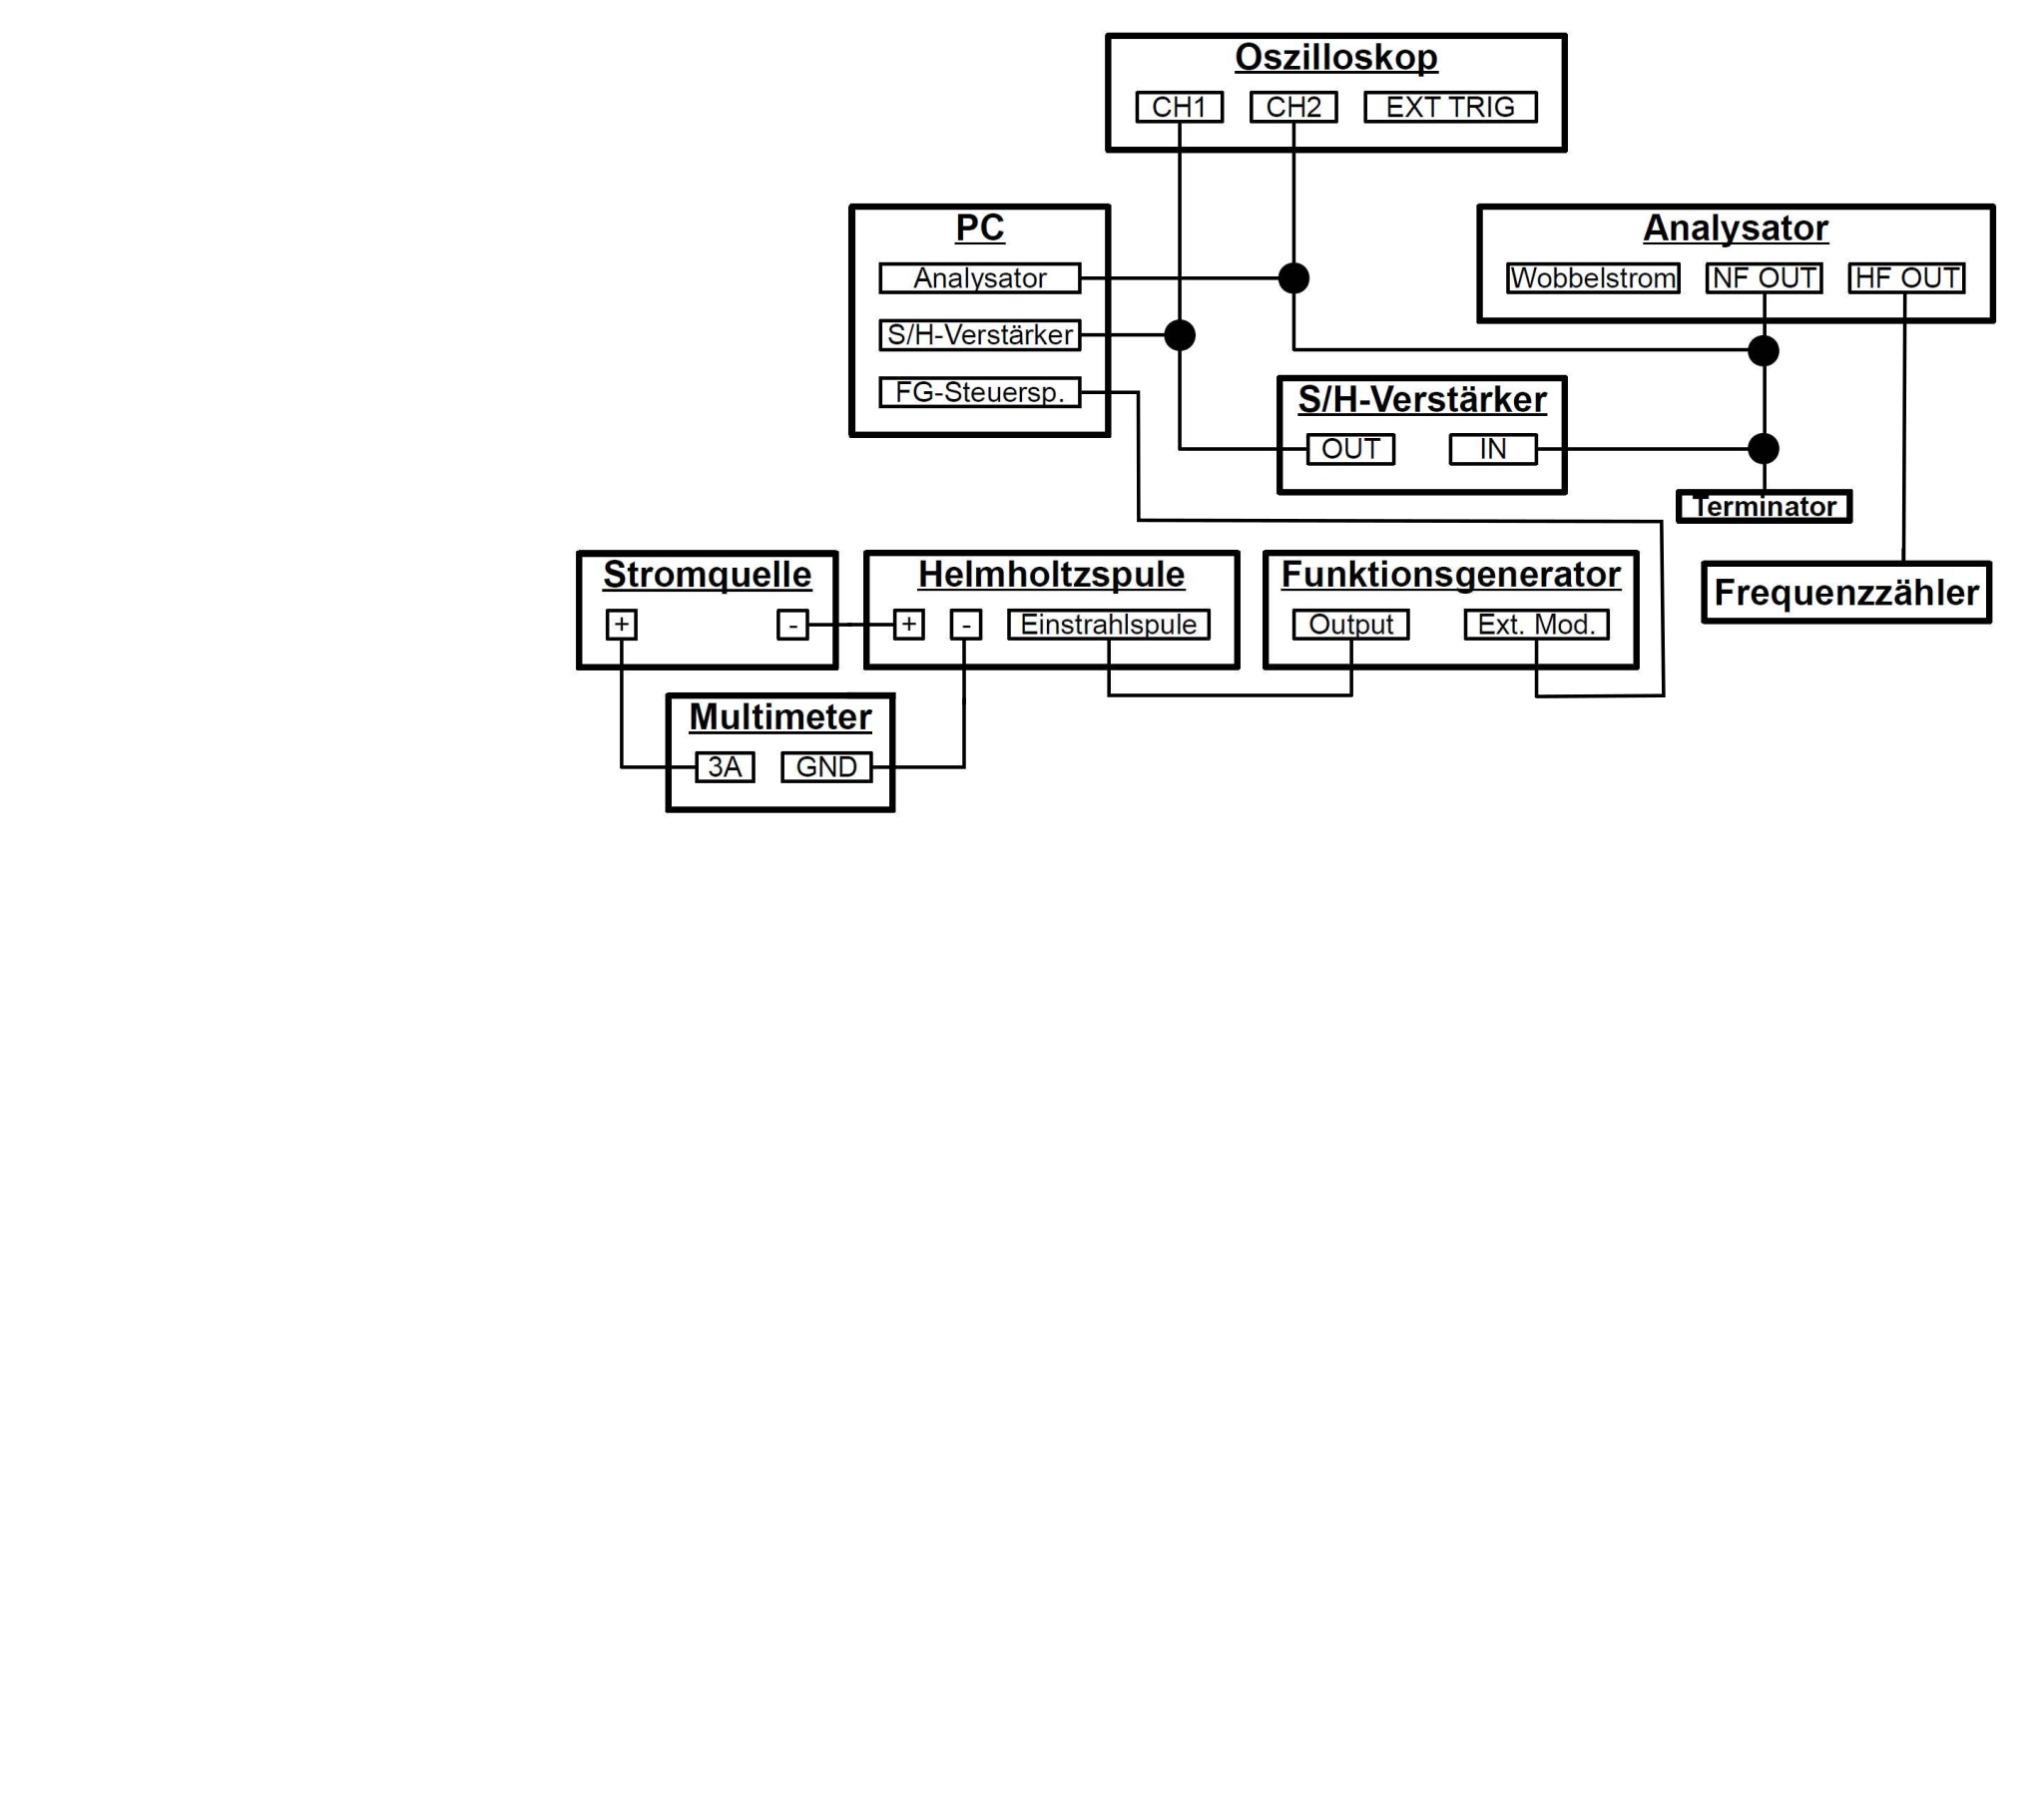
\includegraphics[width=\columnwidth]{Bilder/messbeschaltung.pdf}
	\caption{Beschaltung des gesamten Messaufbaus. Auszüge aus~\citet{anleitung}.}
	\label{fig.beschaltung}
\end{figure}


% =============================================================================
\section{Versuchsdurchführung}
\label{durchfuehrung}
% =============================================================================
%
% ~~~~~~~~~~~~~~~~~~~~~~~~~~~~~~~~~~~~~~~~~~~~~~~~~~~~~~~~~~~~~~~~~~~~~~~~~~~~~
\subsection{Inbetriebnahme des Funktionsgenerators}
\label{vorbereitung1}

\begin{compactitem}
	\item Geräte überprüfen
	\item Vergleich Funktionsgenerator mit Oszillograph
	\item[\tra] führt zu Korrekturfaktoren
	\item Verglich Funktionsgenerator mit Oszillograph bei angeschlossener Einstrahlspule \--- Vorwiderstand \SI{47}{\ohm} Ausgangswiderstand \SI{50}{\ohm}
	\item[\tra] liefert Eichfaktor \--- Funktionsgenerator/Einstrahlspule
\end{compactitem}
% ~~~~~~~~~~~~~~~~~~~~~~~~~~~~~~~~~~~~~~~~~~~~~~~~~~~~~~~~~~~~~~~~~~~~~~~~~~~~~

% ~~~~~~~~~~~~~~~~~~~~~~~~~~~~~~~~~~~~~~~~~~~~~~~~~~~~~~~~~~~~~~~~~~~~~~~~~~~~~
\subsection{Inbetriebnahme Wasserkreislauf, Polaristor und Analysator}
\label{vorbereitung2}

\begin{compactitem}
	\item Pumpe und Polarisationsstrom anschalten (Helmholtz und Manipulation aus)
	\item Analysator anschalten
	\item Signal des Detektors (Analysator/Schwingkreis) anschauen
	\item Ziel: Resonanzfall finden; Ändern der Frequenz des Schwingkreises bis Peaks sichtbar
\end{compactitem}
% ~~~~~~~~~~~~~~~~~~~~~~~~~~~~~~~~~~~~~~~~~~~~~~~~~~~~~~~~~~~~~~~~~~~~~~~~~~~~~

% ~~~~~~~~~~~~~~~~~~~~~~~~~~~~~~~~~~~~~~~~~~~~~~~~~~~~~~~~~~~~~~~~~~~~~~~~~~~~~
\subsection{Inbetriebnahme Computer und Messung von $S2(t_{12})$}
\label{vorbereitung3}



\begin{compactitem}
	\item Messung von $S(t)$ und Resonanzfrequenz bei verschiedenen Impulsabständen $t_{12}$
	\item[d.h.] Resonanzfall finden und leicht verstellen + schauen was passiert \--- Abstände der Peaks
	\item Signal mit und ohne Terminator betrachten
	\item Frequenz des Schwingkreises ändern + zehn Aufnahmen mit dem Computer \--- Frequenz notieren!
	\item schrittweise Änderung der Analysatorspule \--- Aufnahme der Zeitdifferenz der Peaks
	\item[\tra] Resonanzfrequenz bei $t_{12} = \SI{10}{\milli\second}$
	\item[\Tra] Energieaufspaltung und Magnetfeld im Analysator
\end{compactitem}
% ~~~~~~~~~~~~~~~~~~~~~~~~~~~~~~~~~~~~~~~~~~~~~~~~~~~~~~~~~~~~~~~~~~~~~~~~~~~~~

% ~~~~~~~~~~~~~~~~~~~~~~~~~~~~~~~~~~~~~~~~~~~~~~~~~~~~~~~~~~~~~~~~~~~~~~~~~~~~~
\subsection{Inbetriebnahme Sample and Hold Verstärker und Messung von $S2(t,I_{\rm pol})$}
\label{vorbereitung4}

\begin{compactitem}
	\item Anschließen Sample and Hold Verstärker
	\item Einstellen der Phase über Oszillograph auf $S2$ und Messung von $S2(t)$ verschiedenen Polaristionsströmen $I_{\rm pol}$
	\item[\tra] Abhängigkeit der Höhe von $S2(t)$ von der Polarisationsstromstärke $I_{\rm pol}$
	\item Messung Polarisationsstrom und Magnetfeld mit Hall-Sonde \tra linearer Zusammenhang
	\item[\tra] Linearität von Magnetfeld zur Signalhöhe
\end{compactitem}
% ~~~~~~~~~~~~~~~~~~~~~~~~~~~~~~~~~~~~~~~~~~~~~~~~~~~~~~~~~~~~~~~~~~~~~~~~~~~~~
% ~~~~~~~~~~~~~~~~~~~~~~~~~~~~~~~~~~~~~~~~~~~~~~~~~~~~~~~~~~~~~~~~~~~~~~~~~~~~~
\subsection{Messung der Spindrehung im Störfeld, $S2(\nu)$}
\label{vorbereitung5}

\begin{compactitem}
	\item Anschließen Einstrahlspule und Funktionsgenerator
	\item Suchen der Resonanz im Störfeld und Messung der Resonanz im Phasenraum
	\item Protonen im Erdmagnetfeld Larmorfrequenz $\approx \SI{1.2}{\kilo\hertz}$
	\item Funktionsgenerator Amplitude \SI{50}{\milli\volt}
	\item[\tra] Spektrum aufnehmen mit Frequenzgrenzen, dass \SI{1000}{\hertz} durchgefahren wird \--- Durchlaufzeit ca. \SI{60}{\second}
	\item Messung in anderen Frequenzintervallen ober- und unterhalb der Resonanzfrequenz im Erdmagnetfeld 
	\item[\tra] Resonanzfrequenz außerhalb berechneten Stelle \--- Warum?
	\item Messung bei steigender und fallender Frequenz \tra 2 verschobenen, richtige in der Mitte
	\item Amplitude auf \SI{20}{\milli\volt} und Frequenzbereich auch \SI{200}{\hertz}
	\item Resonanzkurven in mehreren Frequenzfenster ohne Bereichsänderung mit Amplituden von $10-\SI{100}{\milli\volt}$ im Abstand von \SI{5}{\milli\volt}
	\item Wann Resonanzpeak besonders deutlich
	\item[\tra] Auflösung des Phasenraums in Amplitude und Frequenz
	\item Resonanzfrequenz genau einstellen, Amplitudenbereich so, dass möglichst viele Spindrehungen zu sehen
	\item[\tra] Aufnahme der Spindrehung in Abhängigkeit der Amplitude
\end{compactitem}
% ~~~~~~~~~~~~~~~~~~~~~~~~~~~~~~~~~~~~~~~~~~~~~~~~~~~~~~~~~~~~~~~~~~~~~~~~~~~~~


% ~~~~~~~~~~~~~~~~~~~~~~~~~~~~~~~~~~~~~~~~~~~~~~~~~~~~~~~~~~~~~~~~~~~~~~~~~~~~~
\subsection{Messung der Resonanz im Feld der Helmholtzspulen}
\label{vorbereitung6}

\begin{compactitem}
	\item 
\end{compactitem}
% ~~~~~~~~~~~~~~~~~~~~~~~~~~~~~~~~~~~~~~~~~~~~~~~~~~~~~~~~~~~~~~~~~~~~~~~~~~~~~
% ~~~~~~~~~~~~~~~~~~~~~~~~~~~~~~~~~~~~~~~~~~~~~~~~~~~~~~~~~~~~~~~~~~~~~~~~~~~~~
\subsection{Bestimmung der Relaxationszeit von Protonen}
\label{vorbereitung7}

\begin{compactitem}
	\item Pumpe aus (20s) Messung starten \--- 2s Pumpe wieder an
	\item Stärke Signal in Abhängigkeit der Pumpleistung messen
	\item[\tra] Relaxationszeit
\end{compactitem}
% ~~~~~~~~~~~~~~~~~~~~~~~~~~~~~~~~~~~~~~~~~~~~~~~~~~~~~~~~~~~~~~~~~~~~~~~~~~~~~
% ~~~~~~~~~~~~~~~~~~~~~~~~~~~~~~~~~~~~~~~~~~~~~~~~~~~~~~~~~~~~~~~~~~~~~~~~~~~~~
\subsection{Bestimmung des Störfeldes}
\label{vorbereitung8}

\begin{compactitem}
	\item Messung der Resonanzfrequenz für positive und negative Helmholtzströme
	\item[\tra] Störfeld
\end{compactitem}
% ~~~~~~~~~~~~~~~~~~~~~~~~~~~~~~~~~~~~~~~~~~~~~~~~~~~~~~~~~~~~~~~~~~~~~~~~~~~~~


%
% =============================================================================
\section{Auswertung}
\label{auswertung}
% =============================================================================
%
% ~~~~~~~~~~~~~~~~~~~~~~~~~~~~~~~~~~~~~~~~~~~~~~~~~~~~~~~~~~~~~~~~~~~~~~~~~~~~~
\subsection{Inbetriebnahme des Funktionsgenerators}
\label{auswertung1}

Um die Genauigkeit des Funktionsgenerators zu überprüfen wird dieser mit dem Oszillographen verbunden. Mit den eingestellten Werten von \SI{50}{\milli\volt} bzw. \SI{100}{\milli\volt} in der Amplitude und \SI{1.3}{\kilo\hertz} bzw. \SI{2.6}{\kilo\hertz} in der Frequenz des Funktionsgenerators messen wir das Signal über den Oszillator, der für die Aufnahme mit dem Computer verbunden ist. An die erhaltenen Messsignale fitten wir jeweils eine Cosinus-Funktion um die Schwankung, die durch die diskrete Zeitauflösung zustande kommt, auszugleichen. Der Fehler der Werte ergibt sich aus der Ungenauigkeit in der Amplitude des Funktionsgenerators von \SI{2}{\percent}. Der Fehler der Fitfunktion kann gegen den Fehler in der Amplitude vernachlässigt werden. Für die vier Messungen vergleichen wir jeweils die Spitze/Spitze Werte, die Amplituden und den Effektivwert. Die Werte sind in Tabelle~\ref{tab.funktionsgenerator} aufgelistet.

\begin{table}[htp]
\begin{center}
	\begin{tabular}{cc|ccc}
		\hline
		\multicolumn{2}{c|}{Funktionsgenerator} &\multicolumn{3}{c}{Oszillograph Spannung in \SI{}{\milli\volt}}\\
		\footnotesize Amplitude & \footnotesize Frequenz & \footnotesize Spitze/Spitze & \footnotesize Amplitude & \footnotesize Effektivwert\\
		\hline
		\SI{50}{\milli\volt} & \SI{1.3}{\kilo\hertz} & \SI{50.2(10)}{} & \SI{100.6(20)}{} & \SI{35.55(71)}{}\\
		\SI{50}{\milli\volt} & \SI{2.6}{\kilo\hertz} & \SI{49.9(10)}{} & \SI{99.9(20)}{} & \SI{35.31(71)}{}\\
		\SI{100}{\milli\volt} & \SI{1.3}{\kilo\hertz} & \SI{100.2(20)}{} & \SI{200.2(40)}{} & \SI{70.87(14)}{}\\
		\SI{100}{\milli\volt} & \SI{2.6}{\kilo\hertz} & \SI{100.3(20)}{} & \SI{200.6(40)}{} & \SI{70.93(14)}{}\\
		\hline
	\end{tabular}
	\caption{Vergleich der eingestellten Werte am Funktionsgenerator mit den am Oszilloskop gemessen Daten, sowie die gemessenen Spitze/Spitze Werte, die Amplituden und Effektivwerten.}
	\label{tab.funktionsgenerator}
\end{center}
\end{table}

Aus dem Vergleich der Werte in Tabelle~\ref{tab.funktionsgenerator} ergibt sich im Rahmen der Fehler kein Unterschied zwischen den Werten am Oszillographen und den eingestellten Werten. Anhand der berechneten Werte erkennt man, dass die Genauigkeit des Funktionsgenerators auch bei unterschiedlichen Amplituden und Frequenzen erhalten bleibt.

Die Einstrahlspule im Manipulator besitzt einen kleinen Innenwiderstand. Allerdings ist der Spule um den Strom zu begrenzen und messbar zu machen ein Vorwiderstand von \SI{47}{\ohm} eingebaut~\citep{anleitung}. Aus dem zusätzlichen Ausgangswiderstand des Funktionsgenerator von \SI{50}{\ohm} wird die Amplitude der Ausgangsspannung reduziert~\citep{anleitung}. Um für nachfolgende Messungen einen Eichfaktor $E_{\rm Spule}$ zu erhalten haben wir obige Messung für eine Frequenz von \SI{1.3}{\kilo\hertz} und die Amplituden \SI{10}{\milli\volt}, \SI{20}{\milli\volt}, \SI{50}{\milli\volt}, \SI{100}{\milli\volt}, \SI{200}{\milli\volt} und \SI{500}{\milli\volt} wiederholt. Hierbei haben wir jeweils eine Messung mit und ein ohne angeschlossener Einstrahlspule aufgenommen. Zur Bestimmung des Eichfaktors $E_{\rm Spule}$ haben wir in Abbildung~\ref{fig.eichfaktor} die gemessenen Spannungen mit angeschlossener Spule $U_{\rm ES}$ über die eingestellten Spannungen des Funktionsgenerators $U_{\rm FG}$ aufgetragen.

\begin{figure}[htp]
	\includegraphics[width=\columnwidth]{Data-Plots/03-Effektivwert-es-fg.pdf}
	\caption{Gemessene Spulenspannung an der Einstrahlspule $U_{\rm ES}$ über die eingestellte Spannung am Funktionsgenerators $E_{\rm FG}$ zur Bestimmung des Eichfaktors.}
	\label{fig.eichfaktor}
\end{figure}

Die Werte in Abbildung~\ref{fig.eichfaktor} sind mit den entsprechenden Fehlern in der Amplitude des Funktionsgenerators (\SI{2}{\percent}) aufgetragen. Zur Bestimmung der Steigung haben wir eine ausgleichende Gerade mit Fehlergeraden an die Daten gelegt. Die Fehler des Fits können vernachlässigt werden.
Für den gemessenen Eichfaktor ergibt sich somit
\begin{equation}
	E_{\rm Spule} = \frac{U_{\rm ES}}{U_{\rm FG}} = \SI{0.4839(97)}{}
\end{equation}
Aus den gemessen Werten erkennen wir, dass der Eichfaktor unabhängig von der gemessenen Frequenz der Wechselspannung an der Einstrahlspule ist. Dies ist auch wichtig um den Eichfaktor für spätere Versuche verwenden zu können, da dort an unterschiedlichen Frequenzen gemessen wird.

Der Eichfaktor kann zudem theoretisch aus der Kenntnis der Widerstandswerte bestimmt werden. 
\begin{equation}
	E_{\rm Spule,theo} = \frac{R_{\rm ES}}{R_{\rm FG}+R_{\rm ES}} = \SI{0.4845(97)}{}
\end{equation}
Der Fehler ergibt sich aus dem geschätzten Fehler des Vorwiderstandes von \SI{2}{\percent}.

Aus dem Vergleich des experimentell bestimmten Wertes mit dem berechneten sehen wir im Rahmen der Fehler eine sehr gute Übereinstimmung. Für nachfolgende Messungen verwenden wir somit den aus unserer Messung erhaltenen Eichfaktor.

% ~~~~~~~~~~~~~~~~~~~~~~~~~~~~~~~~~~~~~~~~~~~~~~~~~~~~~~~~~~~~~~~~~~~~~~~~~~~~~

% ~~~~~~~~~~~~~~~~~~~~~~~~~~~~~~~~~~~~~~~~~~~~~~~~~~~~~~~~~~~~~~~~~~~~~~~~~~~~~
\subsection{Inbetriebnahme Wasserkreislauf, Polaristor und Analysator}
\label{auswertung2}

In diesem Versuchsteil sollte bei eingeschalteter Wasserpumpe, Analysator und Polarisator der Schwingkreis des Analysators auf die Resonanzfrequenz eingestellt werden. Das Signal konnten wir über den Oszillographen beobachtet und durch verändern der Frequenz des Schwingkreises so einstellen, dass die erhaltenen Resonanzsignale mit einem äquidistanten Abstand detektiert werden.

% ~~~~~~~~~~~~~~~~~~~~~~~~~~~~~~~~~~~~~~~~~~~~~~~~~~~~~~~~~~~~~~~~~~~~~~~~~~~~~

% ~~~~~~~~~~~~~~~~~~~~~~~~~~~~~~~~~~~~~~~~~~~~~~~~~~~~~~~~~~~~~~~~~~~~~~~~~~~~~
\subsection{Inbetriebnahme Computer und Messung von $S2(t_{12})$}
\label{auswerung3}

Im dritten Versuchsteil soll die Resonanzfrequenz der Protonenspins im Magnetfeld des Analysator-Magneten bestimmt werden.
Daraus lassen sich die magnetische Feldstärke des Analysator-Magneten und die Energieaufspaltung der Protonen-Spins bestimmen.
Wir variieren dazu die Analysatorfrequenz in kleinen Schritten.
Zweimal pro Periode des Wobbelstromes tritt dabei der Resonanzfall im äußeren Feld auf, wie in \cref{wobbel} skizziert ist.
\begin{figure}[htp]
	\begin{center}
		\includegraphics[width=0.7\columnwidth]{Bilder/Wobbel}
		\caption{Die Analysatorfrequenz trifft zweimal pro Periode des Wobbelfeldes die Resonanzfrequenz. Sie bestimmt mit ihrer Höhe den zeitlichen Abstand zweier Resonanzfälle.}
		\label{wobbel}
	\end{center}
\end{figure}
Damit wird deutlich, dass die Resonanzfrequenz und der zeitliche Abstand $t_{12}$ zwischen zwei Resonanzfällen einen Cosinus-Zusammenhang besitzen.
Wie in \cref{t12} messen wir für 10 verschiedene Analysatorfrequenzen den zeitlichen Abstand zweier der Resonanzen aus.
\begin{figure}[htp]
	\begin{center}
		\includegraphics[width=\columnwidth]{Data-Plots/02-Zeitabstaende.pdf}
		\caption{Für jede Frequenz wird der zeitliche Abstand zweier Resonanzereignisse abgelesen.}
		\label{t12}
	\end{center}
\end{figure}
Die Ablesegenauigkeit der Zeitdifferenzen schätzen wir auf $\SI{0.0002}{}$ Sekunden. 
Der Frequenzzähler zeigte während der Messung leicht unterschiedliche Werte im Bereich von $\SI{\pm 1}{\hertz}$ an.
Diese Unsicherheit vernachlässigen wir gegenüber der Ablesegenauigkeit der Zeitdifferenzen.
Nun tragen wir die Frequenzen über die abgelesenen Zeitdifferenzen  in \cref{resonanzfrequenz} auf und lesen bei $\SI{0.01}{\second}$ die Resonanzfrequenz der Protonen im Feld des Dauermagneten ab.
\begin{align}
	\nu_{\mathrm{res}}=\SI{4712.31\pm 0.20}{\kilo\hertz}
\end{align}
Der Fehler der Resonanzfrequenz ergibt sich auch der Unsicherheit der Zeitdifferenz und der Steigung der Fit-Kurve im Ablesepunkt.
\begin{figure}[htp]
	\begin{center}
		\includegraphics[width=\columnwidth]{Data-Plots/02-Resonanzfrequenz.pdf}
		\caption{Abgelesene Zeitdifferenzen sind in Abhängigkeit der Frequenz aufgetragen und besitzen eine Cosinus-Abhängikeit.}
		\label{resonanzfrequenz}
	\end{center}
\end{figure}
Die Energieaufspaltung und die Magnetfeldstärke des Dauermagneten ergeben sich nun zu
\begin{align}
	\Delta E =h\nu_{\mathrm{res}}=\SI[separate-uncertainty=false]{19.48854(83) e-9}{\eV}
\end{align}
und
\begin{align}
	B_0=\frac{2 \pi \nu_{\mathrm{res}}}{\gamma_p}=\SI[separate-uncertainty=false]{0.1106761(47)}{\tesla}
\end{align}
%\begin{compactitem}
%	\item Messung von $S(t)$ und Resonanzfrequenz bei verschiedenen Impulsabständen $t_{12}$
%	\item[d.h.] Resonanzfall finden und leicht verstellen + schauen was passiert \--- Abstände der Peaks
%	\item Signal mit und ohne Terminator betrachten
%	\item Frequenz des Schwingkreises ändern + zehn Aufnahmen mit dem Computer \--- Frequenz notieren!
%	\item schrittweise Änderung der Analysatorspule \--- Aufnahme der Zeitdifferenz der Peaks
%	\item[\tra] Resonanzfrequenz bei $t_{12} = \SI{10}{\milli\second}$
%	\item[\Tra] Energieaufspaltung und Magnetfeld im Analysator
%\end{compactitem}


% ~~~~~~~~~~~~~~~~~~~~~~~~~~~~~~~~~~~~~~~~~~~~~~~~~~~~~~~~~~~~~~~~~~~~~~~~~~~~~

% ~~~~~~~~~~~~~~~~~~~~~~~~~~~~~~~~~~~~~~~~~~~~~~~~~~~~~~~~~~~~~~~~~~~~~~~~~~~~~
\subsection{Inbetriebnahme Sample and Hold Verstärker und Messung von $S2(t,I_{\rm pol})$}
\label{auswertung4}

Unser Versuchsaufbau wird nun um den S/H-Verstärker erweitert. Mit dem S/H-Verstärker kann nun die Signalhöhe der Resonanzpeaks $S2(t)$ ausgelesen werden. Im folgendem Versuchsteil soll die Abhängigkeit der Signalhöhe von der Polarisationsstromstärke $I_{\rm pol}$ des Polarisators, also der Polarisierung der Protonen im Wasser untersucht werden. Hierfür nehmen wir das Signal $S2(t)$ über die Zeit von \SI{50}{\second} für Polarisationsstöme von \SI{1.3}{\ampere} bis \SI{2.5}{\ampere} in \SI{0.2}{\ampere}-Schritten auf.

Zur Verifikation des Magnetfeldes im Polarisator messen wir mit einer Hall-Sonde das Magnetfeld bei \SI{2.5}{\ampere}. Die Messung mit der Hallsonde beträgt
\begin{equation}
	U_{\rm pol}(\SI{2.5}{\ampere}) = \SI{5.60(5)}{\milli\volt},
\end{equation}
wobei sich der Fehler aus der Ablesegenauigkeit der analogen Spannungsanzeige ergibt. Da der Strom und das Feld im Magneten proportional sind, kann jeder eingestellten Stromstärke am Polarisator eine Magnetfeldstärke zugeordnet werden. Der Fehler des eingestellten Stroms am Polarisatormagneten wird mit \SI{2}{\percent} Anzeigegenauigkeit abgeschätzt.
Um die Linearität des Messsignals in Abhängigkeit vom Magnetfeld zu untersuchen sind die gemessenen Werte in Abbildung~\ref{fig.polarisationsstrom} abgebildet. Die Werte für die Signalhöhe ergeben sich aus einen linearen Fig an die Messdaten der über die Zeit von \SI{50}{\second} aufgenommen Messungen für verschiedene Stromstärken.

\begin{figure}[htp]
	\begin{center}
		\includegraphics[width=\columnwidth]{Data-Plots/04-signal-polarisationsstrom.pdf}
		\caption{Signalhöhe $S2$ der Resonanzpeaks in Abhängigkeit der Polarisationsfeldstärke zur Untersuchung der Linearität.}
		\label{fig.polarisationsstrom}
	\end{center}
\end{figure}

Mit Abbildung~\ref{fig.polarisationsstrom} können wir die Linearität des Messsignals $S2$ zur Polarisationsstromstärke $I_{\rm pol}$ sehr gut bestätigen. Die Fehler im $B$-Feld ergeben sich aus der Ungenauigkeit der Strommessung am Polarisator von \SI{2}{\percent} und der Bestimmung des Magnetfeldes mit der Hallsonde. Der Fehler im Messsignal schätzen wir auf \SI{4}{\percent}. Durch die Anzahl der Messungen können statistische Schwankungen vernachlässigt werden. Der Fehler resultiert somit nur aus der Ungenauigkeit in der Einstellung der Resonanz, sowie der Phase des S/H-Verstärkers.
% ~~~~~~~~~~~~~~~~~~~~~~~~~~~~~~~~~~~~~~~~~~~~~~~~~~~~~~~~~~~~~~~~~~~~~~~~~~~~~
% ~~~~~~~~~~~~~~~~~~~~~~~~~~~~~~~~~~~~~~~~~~~~~~~~~~~~~~~~~~~~~~~~~~~~~~~~~~~~~
\subsection{Messung der Spindrehung im Störfeld, $S2(\nu)$}
\label{auswertung5}
% ~~~~~~~~~~~~~~~~~~~~~~~~~~~~~~~~~~~~~~~~~~~~~~~~~~~~~~~~~~~~~~~~~~~~~~~~~~~~~


% ~~~~~~~~~~~~~~~~~~~~~~~~~~~~~~~~~~~~~~~~~~~~~~~~~~~~~~~~~~~~~~~~~~~~~~~~~~~~~
\subsection{Messung der Resonanz im Feld der Helmholtzspulen}
\label{auswertung6}

% ~~~~~~~~~~~~~~~~~~~~~~~~~~~~~~~~~~~~~~~~~~~~~~~~~~~~~~~~~~~~~~~~~~~~~~~~~~~~~
% ~~~~~~~~~~~~~~~~~~~~~~~~~~~~~~~~~~~~~~~~~~~~~~~~~~~~~~~~~~~~~~~~~~~~~~~~~~~~~
\subsection{Bestimmung der Relaxationszeit von Protonen}
\label{auswertung7}

% ~~~~~~~~~~~~~~~~~~~~~~~~~~~~~~~~~~~~~~~~~~~~~~~~~~~~~~~~~~~~~~~~~~~~~~~~~~~~~
% ~~~~~~~~~~~~~~~~~~~~~~~~~~~~~~~~~~~~~~~~~~~~~~~~~~~~~~~~~~~~~~~~~~~~~~~~~~~~~
\subsection{Bestimmung des Störfeldes}
\label{auswertung8}

% ~~~~~~~~~~~~~~~~~~~~~~~~~~~~~~~~~~~~~~~~~~~~~~~~~~~~~~~~~~~~~~~~~~~~~~~~~~~~~


%
% =============================================================================
\section{Zusammenfassung}
% =============================================================================
%
Wir konnten mit dem Versuch einen guten Einblick in die Röntgenspektroskopie
gewinnen. Die charakteristischen Linien von Eisen, Molybdän und Kupfer wurden mit
recht hoher Genaugikeit nachgewiesen, wobei der größte Abstand von unseren
Bestwerten zu den Theoriewerten 
\SI{0.65}{\percent} betrag. Im Rahmen der Fehler gab es keine Abweichung. 
 Das empirische Gesetz zwischen der Intensität der
charakteristischen Strahlung und der Spannung zeigt systematische Abweichungen
für Spannungen ab \SI{30}{\kilo\volt} und sollte eher als Faustregel verstanden
werden. Das Duane-Hunt-Gesetz hingegen konnte gut bestätigt werden und hat uns
erlaubt, das Plancksche Wirkungsquantum zu bestimmen. Das Moseley-Gesetz wurde
ausführlich diskutiert und hat gute Abschätzungen für die Rydberg-Konstante
ergeben. Allerdings ist die Auswertung der \emph{Abschirmkonstante} $\sigma(Z)$
nicht wirklich sinnvoll. Mit dem Compton-Effekt konnte eine überraschend gute
Bestimmung der Compton-Wellenlänge durchgeführt werden. Eine vollständige
Aufnahme des Transmissionsspektrums von Al im gesamten Wellenlängenbereich der
Kupferanode würde helfen zu verstehen, warum die Näherung eines linearen
Spektrums solch gute Ergebnisse liefert. Die Laue-Aufnahme hat insgesamt gut
funktioniert. Allerdings könnte man die Aufhängung der Dentalfilme zum Beispiel
mit einer optischen Bank o.Ä. verbessern. Dadurch wird ein zentrales 
Auftreffen garantiert. Die Auflösung 
der Filme ist gut, eine größere Fläche wäre zwar wünschenswert, ist für die
Auswertung aber nicht unbedingt notwendig. 
%
% =============================================================================
%\begin{thebibliography}{}   
%% =============================================================================
%%
%%
%  \bibitem{levitt} Levitt, Malcolm H. (2008): Spin dynamics. Basics of nuclear magnetic resonance. 2nd ed. Chichester, England, Hoboken, NJ: John Wiley \& Sons.
%    \bibitem{hanson} Lars G. Hanson (2008): Is Quantum Mechanics Necessary for Understanding Magnetic Resonance?
%    Danish Research Centre for Magnetic Resonance, Copenhagen University Hospital, Hvidovre, Denmark.
%
%\end{thebibliography}
%
%

\small
\bibliographystyle{dinat}
\nocite{*}
\bibliography{lit}
\normalsize


\onecolumn
\pagestyle{empty}
% 

%=============================================================================
\section{Anhang}
\label{Anhang}
% =============================================================================

\end{document}
